\documentclass[11pt]{article}

\usepackage[margin=1in]{geometry}
\usepackage{authblk}
\usepackage{booktabs}
\usepackage{graphicx}
\usepackage{hyperref}
\usepackage{microtype}
\usepackage[numbers,sort&compress]{natbib}
\usepackage{siunitx}
\usepackage{xcolor}

\hypersetup{
  colorlinks=true,
  linkcolor=blue!50!black,
  citecolor=blue!50!black,
  urlcolor=blue!50!black
}

\title{Installed Packages as Context: Package-Scoped Agent Skills for Materials and Chemistry Software}

\author[1]{Author information to be added}
\affil[1]{Affiliation to be added}

\date{Draft ChemRxiv preprint, \today}

\begin{document}

\maketitle

\begin{abstract}
General-purpose coding agents can write syntactically plausible scientific Python, but domain work in materials science and chemistry depends on specialized packages, conventions, and validation checks that are not visible from a natural-language prompt alone. We introduce an environment-aware skills layer that treats installed Python packages as an expression of user intent. Given an environment containing packages such as ASE, pymatgen, RDKit, MACE, impedance.py, py4DSTEM, HyperSpy, PyBaMM, PySCF, OpenMM, matminer, and atomate2, the system selects compact package-scoped \texttt{SKILL.md} files that describe when to use each package, canonical workflows, gotchas, anti-patterns, and diagnostic checks. This package-scoped approach differs from workflow-scoped skill libraries: instead of pre-baking every possible scientific pipeline, it exposes package entry points that can be composed at run time according to the user's actual stack. In a 36-task hidden-rubric evaluation across 12 materials and chemistry packages, package skills improved the aggregate score from 109/180 rubric points for a baseline agent to 165/180 points with package-skill context. Gains were largest for lower-visibility workflow and materials-informatics packages, including atomate2 and matminer. These results support installed environments as a practical source of context for steering scientific coding agents toward domain-specific software rather than generic numerical code.
\end{abstract}

\noindent\textbf{Keywords:} agent skills; scientific Python; materials informatics; computational chemistry; AI coding agents; package metadata; reproducible workflows

\section{Introduction}

Computational science is organized around tasks, workflows, and software packages. A materials scientist may ask for a relaxation, a phase diagram, an equivalent-circuit fit, or a battery discharge simulation; the scientifically correct implementation is rarely just ``use Python.'' It requires choosing the right package, respecting package-specific data models, and applying domain validation checks. In materials science and chemistry, those choices often distinguish a useful answer from a plausible but incorrect generic script: an electrochemical impedance spectrum should not be fit with an unconstrained \texttt{scipy.optimize} model when an equivalent-circuit package is installed; a 4D-STEM datacube should not be reduced to arbitrary NumPy axes before calibration; a materials workflow should not be replaced by a hand-written shell loop when a workflow engine is already in the user's environment.

General coding agents have become increasingly capable at producing code, but scientific coding is not only code generation. It is also package selection, convention selection, and provenance management. Domain packages encode community knowledge in their APIs and tutorials: ASE centers atomistic workflows on \texttt{Atoms} and calculators; pymatgen encodes compositions, structures, symmetry, and phase stability; RDKit encodes molecular graph semantics; PySCF encodes electronic-structure conventions such as basis sets, charge, and spin. When these packages are installed, the user has already revealed substantial information about the conventions likely to apply. Current agents generally underuse this signal.

Recent work on agent steering has converged on ``skills'': filesystem resources containing instructions, references, and optional scripts that a model can load when relevant. Anthropic describes Agent Skills as reusable resources that provide domain-specific expertise, workflows, context, and best practices to general-purpose agents~\cite{anthropic-agent-skills-docs,anthropic-skills-blog,anthropic-skills-explained}. Community projects have begun to collect scientific skills, including K-Dense's open repository of scientific and research skills~\cite{kdense-skills}, while scientific-agent systems such as SciAgent, SciToolAgent, and K-Dense Analyst explore tool-augmented and multi-agent scientific reasoning~\cite{sciagent-2024,scitoolagent-2025,kdense-analyst-2025}. These efforts show the promise of steerable scientific agents, but many skills are workflow-shaped: they describe complete pipelines, domain tasks, or institutional procedures.

We argue for a complementary unit of skill design: \emph{package-scoped skills}. A package-scoped skill is small, composable, and aligned to an installed library. It tells the agent when to reach for the package, how to start from canonical objects, which alternatives are appropriate, and what diagnostics must be checked. This is different from a skill for ``battery modeling workflow'' or ``4D-STEM strain mapping workflow.'' Instead, a PyBaMM skill, a py4DSTEM skill, an ASE skill, and a MACE skill can be composed as the user's installed environment demands. The design bet is that the user's environment is not incidental metadata; it is a latent declaration of scientific intent.

Here we present a prototype environment-aware skills layer for materials and chemistry Python. The contribution is threefold: (i) a package-scoped skill format for scientific Python packages, (ii) an environment-driven discovery mechanism that maps installed packages to skills, and (iii) an empirical hidden-rubric evaluation showing that package skills steer a general coding agent toward domain-specific software and away from generic numerical implementations.

\section{System design}

The prototype has two separable components. First, a registry maps Python distributions to package-scoped skill directories. For example, detecting \texttt{mace-torch} implies the \texttt{mace} skill, while detecting \texttt{rdkit} or \texttt{rdkit-pypi} implies the RDKit skill. Second, each skill is a compact \texttt{SKILL.md} file with structured metadata and sections for use cases, canonical workflow, gotchas, anti-patterns, diagnostics, and deeper references.

The skills are intentionally not documentation mirrors. They are short steering artifacts that point to official documentation and tutorials. A good package skill answers questions that generic API documentation often does not: when should the agent use this package instead of another, what silent failure modes are common, what units and conventions matter, and what outputs should be checked before trust. This keeps the skill small enough to fit in agent context while still preserving the scientific judgment encoded by maintainers' tutorials, papers, and issue patterns.

The current prototype includes 12 package skills: ASE, pymatgen, RDKit, MACE, impedance.py, py4DSTEM, HyperSpy, PyBaMM, PySCF, OpenMM, matminer, and atomate2. These packages span atomistic simulation, materials analysis, cheminformatics, machine-learned interatomic potentials, electrochemistry, electron microscopy, battery modeling, quantum chemistry, molecular dynamics, materials descriptors, and workflow automation.

\section{Evaluation design}

We evaluated whether package skills improve an agent's behavior on realistic package-selection problems. The evaluation contains 36 tasks: three tasks per package across the 12 active skills. Each task is a user-facing scientific coding prompt paired with a hidden rubric. Prompts follow six constraints: (i) the target package name is not visible in the prompt, (ii) only realistic user intent is shown, (iii) generic distractors are listed as available packages, (iv) success criteria are hidden from the model, (v) scoring checks whether the model reaches for the correct installed package instead of generic Python, and (vi) each task records documentation sources and hidden keyword groups for static scoring.

The generic distractor environment is \texttt{numpy}, \texttt{pandas}, \texttt{scipy}, \texttt{scikit-learn}, and \texttt{matplotlib}. The baseline agent receives only the task prompt. The package-skill variant receives the same prompt plus the relevant package skill loaded as context. Both variants are scored with the same five-part rubric (Table~\ref{tab:rubric}). Each task contributes five rubric points, so each package suite contributes 15 points and the full benchmark contributes 180 points.

\begin{table}[htbp]
\centering
\caption{Hidden evaluation rubric used for each domain-specific task.}
\label{tab:rubric}
\begin{tabular}{p{0.08\linewidth}p{0.82\linewidth}}
\toprule
Criterion & Scoring target \\
\midrule
1 & Selects the correct installed domain package instead of a generic numerical or ad hoc implementation. \\
2 & Uses canonical package objects and APIs for the task, rather than treating domain data as raw arrays or tables. \\
3 & Preserves domain representation details such as units, axes, cells, species, frequencies, charges, spin, topology, or metadata. \\
4 & Follows the documented workflow sequence for the package, from input construction through computation and output. \\
5 & Records diagnostics and provenance needed before trusting results, including settings, convergence, residuals, versions, and failure handling. \\
\bottomrule
\end{tabular}
\end{table}

\section{Results}

Package-scoped skills substantially improved aggregate performance. Across 36 tasks, the baseline agent scored 109/180 hidden-rubric points, while the package-skill agent scored 165/180 points. Package skills won 11 of 12 package suites. The only suite-level regression was PySCF, where the baseline scored 14/15 and the package-skill variant scored 13/15 in the full baseline comparison; a subsequent black-box skill-optimization run tied the original PySCF skill at 14/15 and led to adding low-risk guidance about spin conventions and geometry optimization.

Figure~\ref{fig:bar} shows package-level margins. The largest gains were observed for atomate2 and matminer, both +12 rubric points over baseline. These are instructive cases because a generic agent often produced plausible generic workflow or descriptor code, while the package-skill context pointed it to the installed domain package, canonical makers or featurizers, task documents, feature labels, citations, and failure-row audits. Gains were also strong for HyperSpy (+6), PyBaMM (+6), py4DSTEM (+5), impedance.py (+4), pymatgen (+4), and RDKit (+3). More widely known packages such as OpenMM and MACE still improved, but with smaller margins.

\begin{figure}[htbp]
\centering
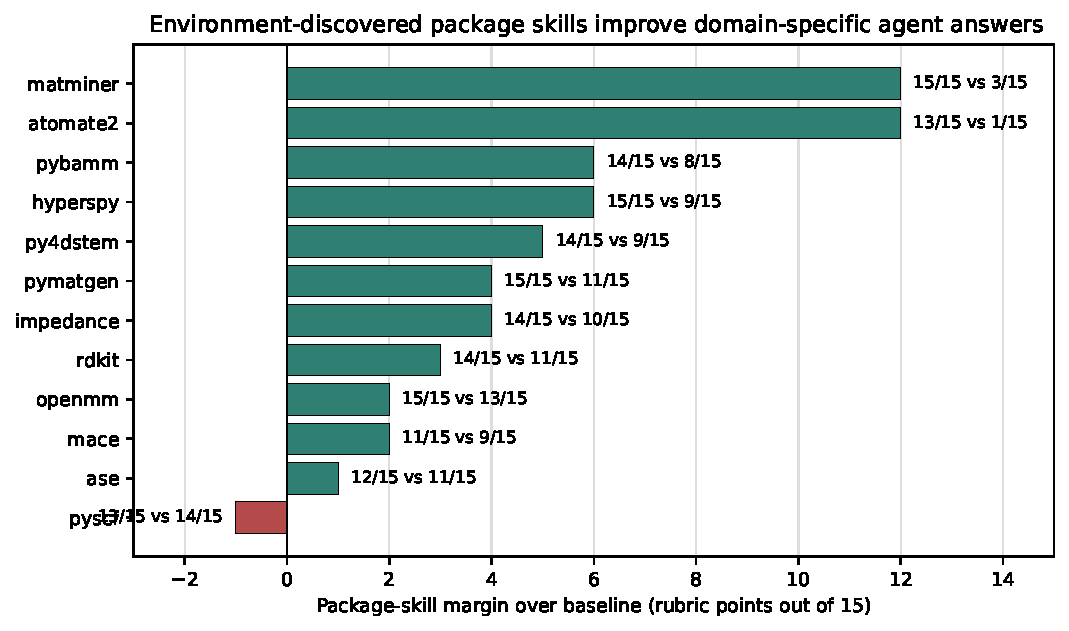
\includegraphics[width=0.95\linewidth]{figures/skill_improvement_bar.pdf}
\caption{Package-skill improvement over baseline for 12 materials and chemistry Python packages. Bars show the difference in hidden-rubric points between the package-skill variant and the baseline agent for each three-task package suite. Each suite has a maximum of 15 points.}
\label{fig:bar}
\end{figure}

We also examined whether package popularity, approximated by GitHub stars, correlated with improvement. Excluding ASE, whose official repository is hosted on GitLab rather than GitHub, the observed correlation between GitHub stars and skill margin was negative in this small sample: Pearson correlation was approximately $-0.48$ for raw stars and $-0.52$ for $\log_{10}$ stars; Spearman correlation was approximately $-0.50$. This is consistent with a saturation interpretation: baseline agents already know more about highly visible packages, so the largest skill gains occur for lower-visibility or more workflow-specific packages. This analysis is exploratory and should not be overinterpreted because the sample contains only 11 GitHub-hosted packages and star counts are an imperfect measure of model familiarity.

\section{Discussion}

The results suggest that package-scoped skills are a useful base unit for exposing open-source scientific software to coding agents. They are smaller than workflow manuals, more composable than pre-baked pipelines, and naturally aligned with the software already present in a user's environment. Installed packages serve as a low-friction context signal: the agent does not need to ask whether the user works with EIS, 4D-STEM, atomistic simulation, cheminformatics, or battery modeling if the environment already contains domain libraries that strongly imply those workflows.

This package-scoped design also creates a practical maintenance path. Package maintainers, research groups, or journals could publish skills alongside documentation. A skill would not replace docs or tutorials; it would be the agent-facing entry point that says: use this package for these tasks, avoid these common mistakes, and check these outputs before making scientific claims. Because skills are plain files, they can be versioned, reviewed, cited, and tested.

The same idea could extend beyond code generation into scientific writing. Journals and preprint servers could eventually publish agent skills for manuscript structure, reporting checklists, figure styles, data-availability language, and discipline-specific conventions. A ChemRxiv style skill, for example, could steer an agent toward appropriate abstract structure, graphical-abstract expectations, figure-label conventions, and chemistry-specific reporting norms. In this framing, skills become a modular interface between scientific communities and agentic drafting systems: communities express standards once, and agents can load them when producing manuscripts, figures, supporting information, or review responses.

Several limitations remain. The evaluation uses static hidden rubrics and one agent/harness rather than executed scientific workflows. The package-skill variant can improve package selection and documented reasoning without guaranteeing executable correctness in every environment. The benchmark currently has only heldout tasks and no train/dev split, so black-box optimization can identify promising skill edits but should not automatically promote changes based on heldout scores alone. Finally, package skills can introduce over-steering: if a task genuinely calls for generic code or a different package, the agent must still reason rather than blindly invoke the installed library.

\section{Conclusion}

Scientific Python environments contain latent user intent. By mapping installed packages to package-scoped skills, agents can be steered toward the domain libraries, workflows, and validation checks that practitioners already use. In a 36-task materials and chemistry benchmark, package skills improved performance from 109/180 to 165/180 hidden-rubric points. The largest gains occurred for domain-specific and workflow-oriented packages that are less likely to be handled correctly by a general coding baseline. Package-scoped skills provide a composable, maintainable mechanism for connecting open-source scientific software to agentic coding and, potentially, agentic scientific writing.

\section*{Data and code availability}

The current prototype, task manifests, skill files, and evaluation artifacts are stored in the accompanying project repository. The draft manuscript uses the evaluation summary in \texttt{eval/extension-score-summary.json} and the generated figure in \texttt{draft-manuscript/figures/skill\_improvement\_bar.pdf}. A public archive DOI should be added before preprint submission.

\section*{Conflicts of interest}

The authors declare no competing financial interests. This statement should be reviewed before submission.

\section*{Acknowledgements}

Acknowledgements should be added before submission. The draft was prepared from local evaluation artifacts and public package documentation.

\begin{thebibliography}{99}

\bibitem{anthropic-agent-skills-docs}
Anthropic. Agent Skills documentation. \url{https://docs.claude.com/en/docs/agents-and-tools/agent-skills}. Accessed May 16, 2026.

\bibitem{anthropic-skills-blog}
Anthropic. Equipping agents for the real world with Agent Skills. \url{https://claude.com/blog/equipping-agents-for-the-real-world-with-agent-skills}. Published October 16, 2025. Accessed May 16, 2026.

\bibitem{anthropic-skills-explained}
Anthropic. Skills explained: How Skills compares to prompts, Projects, MCP, and subagents. \url{https://www.claude.com/blog/skills-explained}. Published November 13, 2025. Accessed May 16, 2026.

\bibitem{kdense-skills}
K-Dense AI. Scientific Agent Skills: a set of ready to use Agent Skills for research, science, engineering, analysis, finance and writing. \url{https://github.com/K-Dense-AI/scientific-agent-skills}. Accessed May 16, 2026.

\bibitem{sciagent-2024}
Chen, Z.; et al. SciAgent: Tool-augmented language models for scientific reasoning. \emph{arXiv} 2024, arXiv:2402.11451. \url{https://arxiv.org/abs/2402.11451}.

\bibitem{scitoolagent-2025}
SciToolAgent: A knowledge graph-driven scientific agent for multi-tool integration. \emph{arXiv} 2025, arXiv:2507.20280. \url{https://arxiv.org/abs/2507.20280}.

\bibitem{kdense-analyst-2025}
K-Dense Analyst: Towards fully automated scientific analysis. \emph{arXiv} 2025, arXiv:2508.07043. \url{https://arxiv.org/abs/2508.07043}.

\bibitem{ase}
Larsen, A. H.; et al. The atomic simulation environment---a Python library for working with atoms. \emph{J. Phys.: Condens. Matter} \textbf{2017}, \emph{29}, 273002. \url{https://doi.org/10.1088/1361-648X/aa680e}.

\bibitem{pymatgen}
Ong, S. P.; et al. Python Materials Genomics (pymatgen): A robust, open-source Python library for materials analysis. \emph{Comput. Mater. Sci.} \textbf{2013}, \emph{68}, 314--319. \url{https://doi.org/10.1016/j.commatsci.2012.10.028}.

\bibitem{rdkit}
RDKit: Open-source cheminformatics. \url{https://www.rdkit.org}. Accessed May 16, 2026.

\bibitem{mace}
Batatia, I.; et al. MACE: Higher order equivariant message passing neural networks for fast and accurate force fields. \emph{arXiv} 2022, arXiv:2206.07697. \url{https://arxiv.org/abs/2206.07697}.

\bibitem{impedance}
Murbach, M. D.; Gerwe, B.; Dawson-Elli, N.; Tsui, L.-k. impedance.py: A Python package for electrochemical impedance analysis. \emph{J. Open Source Softw.} \textbf{2020}, \emph{5}, 2349. \url{https://doi.org/10.21105/joss.02349}.

\bibitem{pybamm}
Sulzer, V.; Marquis, S. G.; Timms, R.; Robinson, M.; Chapman, S. J. Python Battery Mathematical Modelling (PyBaMM). \emph{J. Open Res. Softw.} \textbf{2021}, \emph{9}, 14. \url{https://doi.org/10.5334/jors.309}.

\bibitem{pyscf}
Sun, Q.; et al. PySCF: the Python-based simulations of chemistry framework. \emph{WIREs Comput. Mol. Sci.} \textbf{2018}, \emph{8}, e1340. \url{https://doi.org/10.1002/wcms.1340}.

\bibitem{matminer}
Ward, L.; et al. Matminer: An open source toolkit for materials data mining. \emph{Comput. Mater. Sci.} \textbf{2018}, \emph{152}, 60--69. \url{https://doi.org/10.1016/j.commatsci.2018.05.018}.

\bibitem{openmm}
Eastman, P.; et al. OpenMM 7: Rapid development of high performance algorithms for molecular dynamics. \emph{PLOS Comput. Biol.} \textbf{2017}, \emph{13}, e1005659. \url{https://doi.org/10.1371/journal.pcbi.1005659}.

\bibitem{py4dstem}
py4DSTEM project documentation and repository. \url{https://github.com/py4dstem/py4DSTEM}. Accessed May 16, 2026.

\bibitem{hyperspy}
HyperSpy project documentation and repository. \url{https://github.com/hyperspy/hyperspy}. Accessed May 16, 2026.

\bibitem{atomate2}
Ganose, A. M.; et al. Atomate2: modular workflows for materials science. \emph{Digital Discovery} \textbf{2025}. \url{https://doi.org/10.1039/D5DD00019J}.

\end{thebibliography}

\end{document}
